\section{What makes an Edge?}
\begin{frame}
	\frametitle{What makes an edge?}
	\begin{columns}
		\begin{column}{0.5\textwidth}
			\begin{figure}
				\centering
				
\includegraphics[width=0.8\linewidth]{images/Kadse}
				\caption[Felix]{Felix}
				\label{fig:kadse}
			\end{figure}
		\end{column}
		\begin{column}{0.5\textwidth} 
			\begin{center}
			\begin{figure}
				\centering
				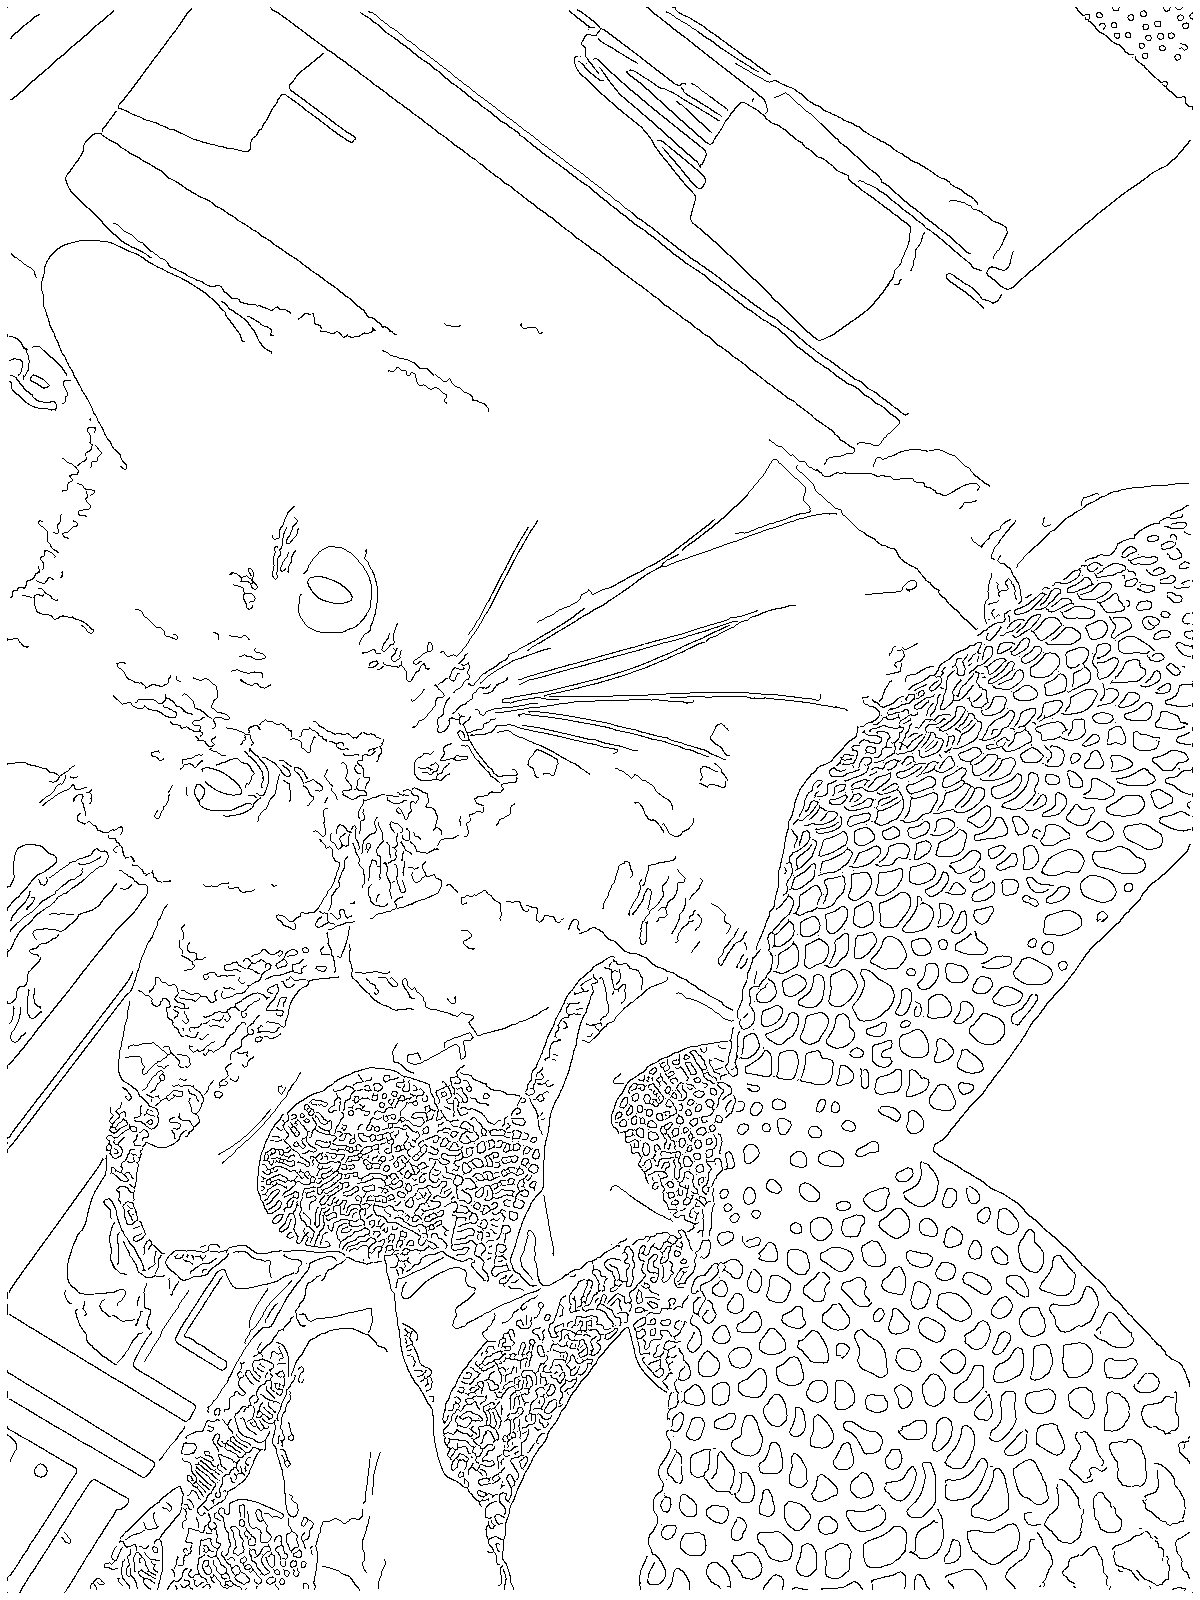
\includegraphics[width=0.8\linewidth]{images/KadseCanny}
				\caption[Felix's Edges]{Felix's Edges}
				\label{fig:kadseCanny}
			\end{figure}
			\end{center}
		\end{column}
	\end{columns}
\end{frame}
\begin{frame}
	\frametitle{Problem I: Contrast}
	\begin{columns}
		\begin{column}{0.5\textwidth}
			\begin{figure}
				\centering
				
\includegraphics[width=0.8\linewidth]{images/KadseHighContrast}
				\caption[High Contrast Felix]{High Contrast Felix}
				\label{fig:HighContrast}
			\end{figure}
		\end{column}
		\begin{column}{0.5\textwidth} 
			\begin{center}
				\begin{figure}
					\centering
					
\includegraphics[width=0.8\linewidth]{images/KadseLowContrast}
					\caption[Low Contrast Felix]{Low Contrast Felix}
					\label{fig:LowContrast}
				\end{figure}
			\end{center}
		\end{column}
	\end{columns}
\end{frame}

\begin{frame}
	\frametitle{Problem II: Smoothness}
	\begin{center}
		\begin{figure}
			\centering
			
\includegraphics[width=0.4\linewidth]{images/KadseSmooth}
			\caption[Smooth Felix]{Smooth Felix}
			\label{fig:Smooth}
		\end{figure}
	\end{center}
\end{frame}

\begin{frame}
	\frametitle{Problem III: Noise}
	\begin{center}
		\begin{figure}
			\centering
			
\includegraphics[width=0.4\linewidth]{images/KadseSalty}
			\caption[Salted Felix]{Salted Felix}
			\label{fig:Salted}
		\end{figure}
	\end{center}
\end{frame}

\begin{frame}
	\frametitle{Definition}
	In Image Processing, an edge can be defined as a set of contiguous pixel positions where an abrupt change of intensity, gray- or color-values occur. Edges represent boundaries between objects and background. Sometimes, the edge-pixel-sequence may be broken due to insufficient intensity difference.(Malay K. Pakhira )
\end{frame}	
